% Created by tikzDevice version 0.12.6 on 2026-08-08 12:11:50
% !TEX encoding = UTF-8 Unicode
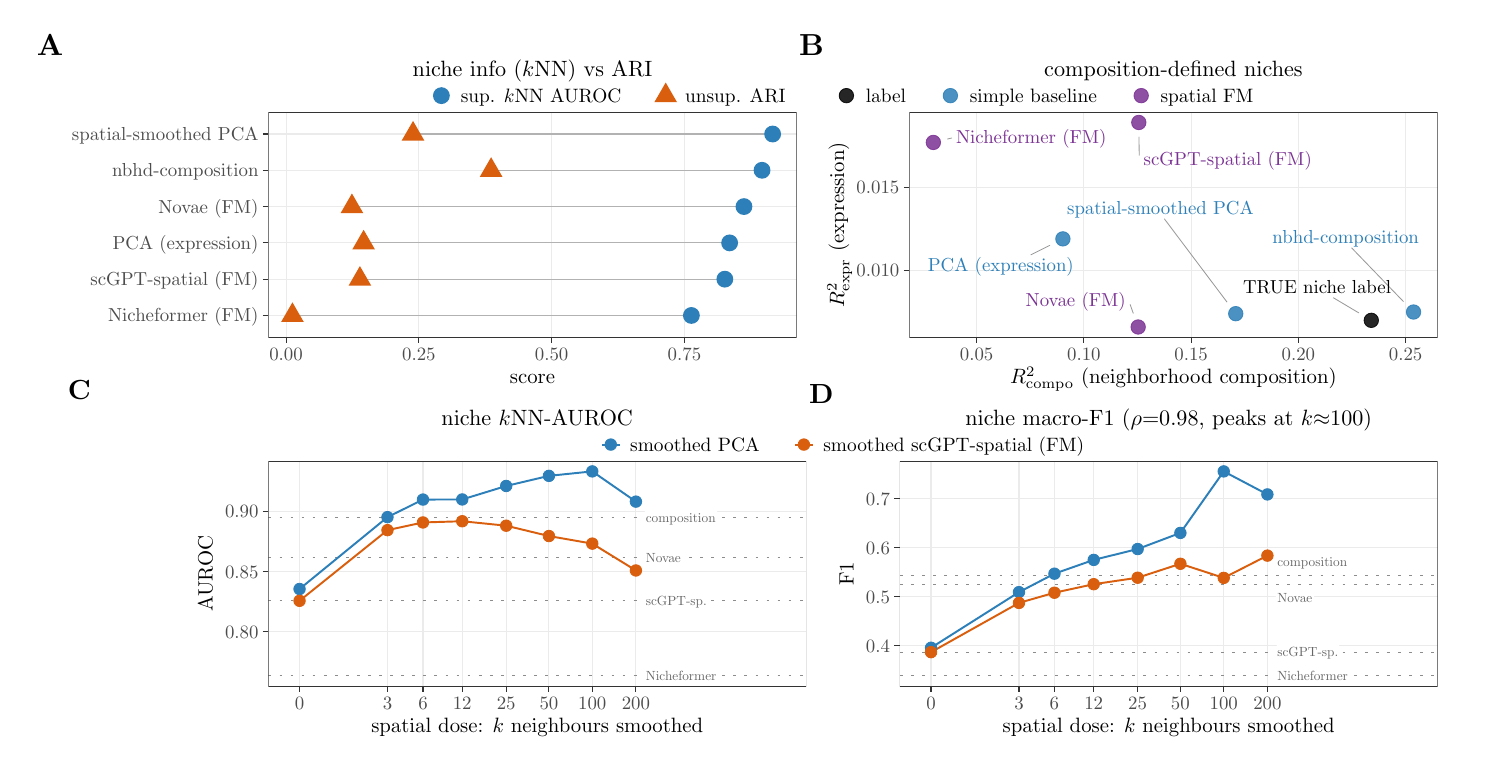
\begin{tikzpicture}[x=1pt,y=1pt]
\definecolor{fillColor}{RGB}{255,255,255}
\path[use as bounding box,fill=fillColor,fill opacity=0.00] (0,0) rectangle (517.45,260.17);
\begin{scope}
\path[clip] (  0.00,  0.00) rectangle (517.45,260.17);
\definecolor{drawColor}{RGB}{255,255,255}
\definecolor{fillColor}{RGB}{255,255,255}

\path[draw=drawColor,line width= 0.4pt,line join=round,line cap=round,fill=fillColor] (  0.00,  0.00) rectangle (517.45,260.17);
\end{scope}
\begin{scope}
\path[clip] (  8.00,128.09) rectangle (281.87,254.17);
\definecolor{drawColor}{RGB}{255,255,255}
\definecolor{fillColor}{RGB}{255,255,255}

\path[draw=drawColor,line width= 0.4pt,line join=round,line cap=round,fill=fillColor] (  8.00,128.09) rectangle (281.87,254.17);
\end{scope}
\begin{scope}
\path[clip] (281.87,128.09) rectangle (513.45,254.17);
\definecolor{drawColor}{RGB}{255,255,255}
\definecolor{fillColor}{RGB}{255,255,255}

\path[draw=drawColor,line width= 0.4pt,line join=round,line cap=round,fill=fillColor] (281.87,128.09) rectangle (513.45,254.17);
\end{scope}
\begin{scope}
\path[clip] ( 87.00,148.31) rectangle (277.87,229.61);
\definecolor{fillColor}{RGB}{255,255,255}

\path[fill=fillColor] ( 87.00,148.31) rectangle (277.87,229.61);
\definecolor{drawColor}{gray}{0.92}

\path[draw=drawColor,line width= 0.4pt,line join=round] ( 87.00,156.18) --
	(277.87,156.18);

\path[draw=drawColor,line width= 0.4pt,line join=round] ( 87.00,169.29) --
	(277.87,169.29);

\path[draw=drawColor,line width= 0.4pt,line join=round] ( 87.00,182.40) --
	(277.87,182.40);

\path[draw=drawColor,line width= 0.4pt,line join=round] ( 87.00,195.52) --
	(277.87,195.52);

\path[draw=drawColor,line width= 0.4pt,line join=round] ( 87.00,208.63) --
	(277.87,208.63);

\path[draw=drawColor,line width= 0.4pt,line join=round] ( 87.00,221.74) --
	(277.87,221.74);

\path[draw=drawColor,line width= 0.4pt,line join=round] ( 93.37,148.31) --
	( 93.37,229.61);

\path[draw=drawColor,line width= 0.4pt,line join=round] (141.36,148.31) --
	(141.36,229.61);

\path[draw=drawColor,line width= 0.4pt,line join=round] (189.34,148.31) --
	(189.34,229.61);

\path[draw=drawColor,line width= 0.4pt,line join=round] (237.33,148.31) --
	(237.33,229.61);
\definecolor{drawColor}{gray}{0.70}

\path[draw=drawColor,line width= 0.4pt,line join=round] ( 95.67,156.18) --
	(239.83,156.18);

\path[draw=drawColor,line width= 0.4pt,line join=round] (120.05,169.29) --
	(251.92,169.29);

\path[draw=drawColor,line width= 0.4pt,line join=round] (121.39,182.40) --
	(253.65,182.40);

\path[draw=drawColor,line width= 0.4pt,line join=round] (117.17,195.52) --
	(258.83,195.52);

\path[draw=drawColor,line width= 0.4pt,line join=round] (167.46,208.63) --
	(265.36,208.63);

\path[draw=drawColor,line width= 0.4pt,line join=round] (139.25,221.74) --
	(269.19,221.74);
\definecolor{fillColor}{RGB}{217,95,14}

\path[fill=fillColor] (167.46,213.36) --
	(171.56,206.26) --
	(163.36,206.26) --
	cycle;

\path[fill=fillColor] (121.39,187.14) --
	(125.49,180.04) --
	(117.30,180.04) --
	cycle;

\path[fill=fillColor] (139.25,226.47) --
	(143.34,219.37) --
	(135.15,219.37) --
	cycle;

\path[fill=fillColor] ( 95.67,160.91) --
	( 99.77,153.82) --
	( 91.57,153.82) --
	cycle;

\path[fill=fillColor] (117.17,200.25) --
	(121.27,193.15) --
	(113.07,193.15) --
	cycle;

\path[fill=fillColor] (120.05,174.03) --
	(124.15,166.93) --
	(115.95,166.93) --
	cycle;
\definecolor{fillColor}{RGB}{44,127,184}

\path[fill=fillColor] (265.36,208.63) circle (  3.04);

\path[fill=fillColor] (253.65,182.40) circle (  3.04);

\path[fill=fillColor] (269.19,221.74) circle (  3.04);

\path[fill=fillColor] (239.83,156.18) circle (  3.04);

\path[fill=fillColor] (258.83,195.52) circle (  3.04);

\path[fill=fillColor] (251.92,169.29) circle (  3.04);
\definecolor{drawColor}{gray}{0.20}

\path[draw=drawColor,line width= 0.4pt,line join=round,line cap=round] ( 87.00,148.31) rectangle (277.87,229.61);
\end{scope}
\begin{scope}
\path[clip] (  0.00,  0.00) rectangle (517.45,260.17);
\definecolor{drawColor}{gray}{0.30}

\node[text=drawColor,anchor=base east,inner sep=0pt, outer sep=0pt, scale=  0.68] at ( 83.40,153.84) {Nicheformer (FM)};

\node[text=drawColor,anchor=base east,inner sep=0pt, outer sep=0pt, scale=  0.68] at ( 83.40,166.95) {scGPT-spatial (FM)};

\node[text=drawColor,anchor=base east,inner sep=0pt, outer sep=0pt, scale=  0.68] at ( 83.40,180.06) {PCA (expression)};

\node[text=drawColor,anchor=base east,inner sep=0pt, outer sep=0pt, scale=  0.68] at ( 83.40,193.17) {Novae (FM)};

\node[text=drawColor,anchor=base east,inner sep=0pt, outer sep=0pt, scale=  0.68] at ( 83.40,206.29) {nbhd-composition};

\node[text=drawColor,anchor=base east,inner sep=0pt, outer sep=0pt, scale=  0.68] at ( 83.40,219.40) {spatial-smoothed PCA};
\end{scope}
\begin{scope}
\path[clip] (  0.00,  0.00) rectangle (517.45,260.17);
\definecolor{drawColor}{gray}{0.20}

\path[draw=drawColor,line width= 0.4pt,line join=round] ( 85.00,156.18) --
	( 87.00,156.18);

\path[draw=drawColor,line width= 0.4pt,line join=round] ( 85.00,169.29) --
	( 87.00,169.29);

\path[draw=drawColor,line width= 0.4pt,line join=round] ( 85.00,182.40) --
	( 87.00,182.40);

\path[draw=drawColor,line width= 0.4pt,line join=round] ( 85.00,195.52) --
	( 87.00,195.52);

\path[draw=drawColor,line width= 0.4pt,line join=round] ( 85.00,208.63) --
	( 87.00,208.63);

\path[draw=drawColor,line width= 0.4pt,line join=round] ( 85.00,221.74) --
	( 87.00,221.74);
\end{scope}
\begin{scope}
\path[clip] (  0.00,  0.00) rectangle (517.45,260.17);
\definecolor{drawColor}{gray}{0.20}

\path[draw=drawColor,line width= 0.4pt,line join=round] ( 93.37,146.31) --
	( 93.37,148.31);

\path[draw=drawColor,line width= 0.4pt,line join=round] (141.36,146.31) --
	(141.36,148.31);

\path[draw=drawColor,line width= 0.4pt,line join=round] (189.34,146.31) --
	(189.34,148.31);

\path[draw=drawColor,line width= 0.4pt,line join=round] (237.33,146.31) --
	(237.33,148.31);
\end{scope}
\begin{scope}
\path[clip] (  0.00,  0.00) rectangle (517.45,260.17);
\definecolor{drawColor}{gray}{0.30}

\node[text=drawColor,anchor=base,inner sep=0pt, outer sep=0pt, scale=  0.68] at ( 93.37,140.03) {0.00};

\node[text=drawColor,anchor=base,inner sep=0pt, outer sep=0pt, scale=  0.68] at (141.36,140.03) {0.25};

\node[text=drawColor,anchor=base,inner sep=0pt, outer sep=0pt, scale=  0.68] at (189.34,140.03) {0.50};

\node[text=drawColor,anchor=base,inner sep=0pt, outer sep=0pt, scale=  0.68] at (237.33,140.03) {0.75};
\end{scope}
\begin{scope}
\path[clip] (  0.00,  0.00) rectangle (517.45,260.17);
\definecolor{drawColor}{RGB}{0,0,0}

\node[text=drawColor,anchor=base,inner sep=0pt, outer sep=0pt, scale=  0.75] at (182.43,131.54) {score};
\end{scope}
\begin{scope}
\path[clip] (  0.00,  0.00) rectangle (517.45,260.17);
\definecolor{drawColor}{RGB}{0,0,0}

\node[text=drawColor,anchor=base,inner sep=0pt, outer sep=0pt, scale=  0.80] at (182.43,242.66) {niche info ($k$NN) vs ARI};
\end{scope}
\begin{scope}
\path[clip] (  0.00,  0.00) rectangle (517.45,260.17);
\definecolor{drawColor}{RGB}{0,0,0}

\node[text=drawColor,anchor=base,inner sep=0pt, outer sep=0pt, scale=  1.10] at (  8.14,250.28) {\bfseries A};
\end{scope}
\begin{scope}
\path[clip] (318.58,148.31) rectangle (509.45,229.61);
\definecolor{fillColor}{RGB}{255,255,255}

\path[fill=fillColor] (318.58,148.31) rectangle (509.45,229.61);
\definecolor{drawColor}{gray}{0.92}

\path[draw=drawColor,line width= 0.4pt,line join=round] (318.58,172.44) --
	(509.45,172.44);

\path[draw=drawColor,line width= 0.4pt,line join=round] (318.58,202.48) --
	(509.45,202.48);

\path[draw=drawColor,line width= 0.4pt,line join=round] (342.91,148.31) --
	(342.91,229.61);

\path[draw=drawColor,line width= 0.4pt,line join=round] (381.66,148.31) --
	(381.66,229.61);

\path[draw=drawColor,line width= 0.4pt,line join=round] (420.41,148.31) --
	(420.41,229.61);

\path[draw=drawColor,line width= 0.4pt,line join=round] (459.16,148.31) --
	(459.16,229.61);

\path[draw=drawColor,line width= 0.4pt,line join=round] (497.91,148.31) --
	(497.91,229.61);
\definecolor{drawColor}{RGB}{0,0,0}
\definecolor{fillColor}{RGB}{0,0,0}

\path[draw=drawColor,draw opacity=0.85,line width= 0.3pt,line join=round,line cap=round,fill=fillColor,fill opacity=0.85] (485.51,154.41) circle (  2.61);
\definecolor{drawColor}{RGB}{44,127,184}
\definecolor{fillColor}{RGB}{44,127,184}

\path[draw=drawColor,draw opacity=0.85,line width= 0.3pt,line join=round,line cap=round,fill=fillColor,fill opacity=0.85] (500.78,157.42) circle (  2.61);

\path[draw=drawColor,draw opacity=0.85,line width= 0.3pt,line join=round,line cap=round,fill=fillColor,fill opacity=0.85] (374.07,183.85) circle (  2.61);

\path[draw=drawColor,draw opacity=0.85,line width= 0.3pt,line join=round,line cap=round,fill=fillColor,fill opacity=0.85] (436.53,156.82) circle (  2.61);
\definecolor{drawColor}{RGB}{123,50,148}
\definecolor{fillColor}{RGB}{123,50,148}

\path[draw=drawColor,draw opacity=0.85,line width= 0.3pt,line join=round,line cap=round,fill=fillColor,fill opacity=0.85] (327.26,218.70) circle (  2.61);

\path[draw=drawColor,draw opacity=0.85,line width= 0.3pt,line join=round,line cap=round,fill=fillColor,fill opacity=0.85] (401.27,152.01) circle (  2.61);

\path[draw=drawColor,draw opacity=0.85,line width= 0.3pt,line join=round,line cap=round,fill=fillColor,fill opacity=0.85] (401.50,225.91) circle (  2.61);
\definecolor{drawColor}{gray}{0.60}

\path[draw=drawColor,line width= 0.3pt,line join=round,line cap=round] (471.81,162.57) -- (480.97,157.12);

\path[draw=drawColor,line width= 0.3pt,line join=round,line cap=round] (478.43,180.57) -- (497.11,161.22);

\path[draw=drawColor,line width= 0.3pt,line join=round,line cap=round] (362.50,178.10) -- (369.33,181.50);

\path[draw=drawColor,line width= 0.3pt,line join=round,line cap=round] (410.74,191.08) -- (433.35,161.04);

\path[draw=drawColor,line width= 0.3pt,line join=round,line cap=round] (333.87,220.29) -- (332.40,219.94);

\path[draw=drawColor,line width= 0.3pt,line join=round,line cap=round] (398.38,160.11) -- (399.49,156.99);

\path[draw=drawColor,line width= 0.3pt,line join=round,line cap=round] (401.65,214.04) -- (401.57,220.63);
\definecolor{drawColor}{RGB}{0,0,0}

\node[text=drawColor,anchor=base,inner sep=0pt, outer sep=0pt, scale=  0.68] at (465.91,164.08) {TRUE niche label};
\definecolor{drawColor}{RGB}{44,127,184}

\node[text=drawColor,anchor=base,inner sep=0pt, outer sep=0pt, scale=  0.68] at (476.26,182.08) {nbhd-composition};

\node[text=drawColor,anchor=base,inner sep=0pt, outer sep=0pt, scale=  0.68] at (351.66,171.89) {PCA (expression)};

\node[text=drawColor,anchor=base,inner sep=0pt, outer sep=0pt, scale=  0.68] at (409.30,192.59) {spatial-smoothed PCA};
\definecolor{drawColor}{RGB}{123,50,148}

\node[text=drawColor,anchor=base,inner sep=0pt, outer sep=0pt, scale=  0.68] at (362.66,218.28) {Nicheformer (FM)};

\node[text=drawColor,anchor=base,inner sep=0pt, outer sep=0pt, scale=  0.68] at (378.71,159.27) {Novae (FM)};

\node[text=drawColor,anchor=base,inner sep=0pt, outer sep=0pt, scale=  0.68] at (433.65,210.54) {scGPT-spatial (FM)};
\definecolor{drawColor}{gray}{0.20}

\path[draw=drawColor,line width= 0.4pt,line join=round,line cap=round] (318.58,148.31) rectangle (509.45,229.61);
\end{scope}
\begin{scope}
\path[clip] (  0.00,  0.00) rectangle (517.45,260.17);
\definecolor{drawColor}{gray}{0.30}

\node[text=drawColor,anchor=base east,inner sep=0pt, outer sep=0pt, scale=  0.68] at (314.98,170.10) {0.010};

\node[text=drawColor,anchor=base east,inner sep=0pt, outer sep=0pt, scale=  0.68] at (314.98,200.14) {0.015};
\end{scope}
\begin{scope}
\path[clip] (  0.00,  0.00) rectangle (517.45,260.17);
\definecolor{drawColor}{gray}{0.20}

\path[draw=drawColor,line width= 0.4pt,line join=round] (316.58,172.44) --
	(318.58,172.44);

\path[draw=drawColor,line width= 0.4pt,line join=round] (316.58,202.48) --
	(318.58,202.48);
\end{scope}
\begin{scope}
\path[clip] (  0.00,  0.00) rectangle (517.45,260.17);
\definecolor{drawColor}{gray}{0.20}

\path[draw=drawColor,line width= 0.4pt,line join=round] (342.91,146.31) --
	(342.91,148.31);

\path[draw=drawColor,line width= 0.4pt,line join=round] (381.66,146.31) --
	(381.66,148.31);

\path[draw=drawColor,line width= 0.4pt,line join=round] (420.41,146.31) --
	(420.41,148.31);

\path[draw=drawColor,line width= 0.4pt,line join=round] (459.16,146.31) --
	(459.16,148.31);

\path[draw=drawColor,line width= 0.4pt,line join=round] (497.91,146.31) --
	(497.91,148.31);
\end{scope}
\begin{scope}
\path[clip] (  0.00,  0.00) rectangle (517.45,260.17);
\definecolor{drawColor}{gray}{0.30}

\node[text=drawColor,anchor=base,inner sep=0pt, outer sep=0pt, scale=  0.68] at (342.91,140.03) {0.05};

\node[text=drawColor,anchor=base,inner sep=0pt, outer sep=0pt, scale=  0.68] at (381.66,140.03) {0.10};

\node[text=drawColor,anchor=base,inner sep=0pt, outer sep=0pt, scale=  0.68] at (420.41,140.03) {0.15};

\node[text=drawColor,anchor=base,inner sep=0pt, outer sep=0pt, scale=  0.68] at (459.16,140.03) {0.20};

\node[text=drawColor,anchor=base,inner sep=0pt, outer sep=0pt, scale=  0.68] at (497.91,140.03) {0.25};
\end{scope}
\begin{scope}
\path[clip] (  0.00,  0.00) rectangle (517.45,260.17);
\definecolor{drawColor}{RGB}{0,0,0}

\node[text=drawColor,anchor=base,inner sep=0pt, outer sep=0pt, scale=  0.75] at (414.02,131.54) {$R^2_{\mathrm{compo}}$ (neighborhood composition)};
\end{scope}
\begin{scope}
\path[clip] (  0.00,  0.00) rectangle (517.45,260.17);
\definecolor{drawColor}{RGB}{0,0,0}

\node[text=drawColor,rotate= 90.00,anchor=base,inner sep=0pt, outer sep=0pt, scale=  0.75] at (295.04,188.96) {$R^2_{\mathrm{expr}}$ (expression)};
\end{scope}
\begin{scope}
\path[clip] (  0.00,  0.00) rectangle (517.45,260.17);
\definecolor{drawColor}{RGB}{0,0,0}

\node[text=drawColor,anchor=base,inner sep=0pt, outer sep=0pt, scale=  0.80] at (414.02,242.66) {composition-defined niches};
\end{scope}
\begin{scope}
\path[clip] (  0.00,  0.00) rectangle (517.45,260.17);
\definecolor{drawColor}{RGB}{0,0,0}

\node[text=drawColor,anchor=base,inner sep=0pt, outer sep=0pt, scale=  1.10] at (283.28,250.28) {\bfseries B};
\end{scope}
\begin{scope}
\path[clip] (  0.00,  0.00) rectangle (517.45,260.17);
\definecolor{fillColor}{RGB}{255,255,255}

\path[fill=fillColor] (144.50,231.61) rectangle (282.84,239.61);
\end{scope}
\begin{scope}
\path[clip] (  0.00,  0.00) rectangle (517.45,260.17);
\definecolor{fillColor}{RGB}{255,255,255}

\path[fill=fillColor] (145.50,231.61) rectangle (153.50,239.61);
\definecolor{fillColor}{RGB}{44,127,184}

\path[fill=fillColor] (149.50,235.61) circle (  3.04);
\end{scope}
\begin{scope}
\path[clip] (  0.00,  0.00) rectangle (517.45,260.17);
\definecolor{fillColor}{RGB}{255,255,255}

\path[fill=fillColor] (226.55,231.61) rectangle (234.55,239.61);
\definecolor{fillColor}{RGB}{217,95,14}

\path[fill=fillColor] (230.55,240.34) --
	(234.64,233.24) --
	(226.45,233.24) --
	cycle;
\end{scope}
\begin{scope}
\path[clip] (  0.00,  0.00) rectangle (517.45,260.17);
\definecolor{drawColor}{RGB}{0,0,0}

\node[text=drawColor,anchor=base west,inner sep=0pt, outer sep=0pt, scale=  0.70] at (156.50,233.20) {sup. $k$NN AUROC};
\end{scope}
\begin{scope}
\path[clip] (  0.00,  0.00) rectangle (517.45,260.17);
\definecolor{drawColor}{RGB}{0,0,0}

\node[text=drawColor,anchor=base west,inner sep=0pt, outer sep=0pt, scale=  0.70] at (237.55,233.20) {unsup. ARI};
\end{scope}
\begin{scope}
\path[clip] (  0.00,  0.00) rectangle (517.45,260.17);
\definecolor{fillColor}{RGB}{255,255,255}

\path[fill=fillColor] (290.84,231.61) rectangle (451.95,239.61);
\end{scope}
\begin{scope}
\path[clip] (  0.00,  0.00) rectangle (517.45,260.17);
\definecolor{fillColor}{RGB}{255,255,255}

\path[fill=fillColor] (291.84,231.61) rectangle (299.84,239.61);
\definecolor{drawColor}{RGB}{0,0,0}
\definecolor{fillColor}{RGB}{0,0,0}

\path[draw=drawColor,draw opacity=0.85,line width= 0.3pt,line join=round,line cap=round,fill=fillColor,fill opacity=0.85] (295.84,235.61) circle (  2.61);
\end{scope}
\begin{scope}
\path[clip] (  0.00,  0.00) rectangle (517.45,260.17);
\definecolor{fillColor}{RGB}{255,255,255}

\path[fill=fillColor] (329.42,231.61) rectangle (337.42,239.61);
\definecolor{drawColor}{RGB}{44,127,184}
\definecolor{fillColor}{RGB}{44,127,184}

\path[draw=drawColor,draw opacity=0.85,line width= 0.3pt,line join=round,line cap=round,fill=fillColor,fill opacity=0.85] (333.42,235.61) circle (  2.61);
\end{scope}
\begin{scope}
\path[clip] (  0.00,  0.00) rectangle (517.45,260.17);
\definecolor{fillColor}{RGB}{255,255,255}

\path[fill=fillColor] (398.37,231.61) rectangle (406.37,239.61);
\definecolor{drawColor}{RGB}{123,50,148}
\definecolor{fillColor}{RGB}{123,50,148}

\path[draw=drawColor,draw opacity=0.85,line width= 0.3pt,line join=round,line cap=round,fill=fillColor,fill opacity=0.85] (402.37,235.61) circle (  2.61);
\end{scope}
\begin{scope}
\path[clip] (  0.00,  0.00) rectangle (517.45,260.17);
\definecolor{drawColor}{RGB}{0,0,0}

\node[text=drawColor,anchor=base west,inner sep=0pt, outer sep=0pt, scale=  0.70] at (302.84,233.20) {label};
\end{scope}
\begin{scope}
\path[clip] (  0.00,  0.00) rectangle (517.45,260.17);
\definecolor{drawColor}{RGB}{0,0,0}

\node[text=drawColor,anchor=base west,inner sep=0pt, outer sep=0pt, scale=  0.70] at (340.42,233.20) {simple baseline};
\end{scope}
\begin{scope}
\path[clip] (  0.00,  0.00) rectangle (517.45,260.17);
\definecolor{drawColor}{RGB}{0,0,0}

\node[text=drawColor,anchor=base west,inner sep=0pt, outer sep=0pt, scale=  0.70] at (409.37,233.20) {spatial FM};
\end{scope}
\begin{scope}
\path[clip] (  8.00,  2.00) rectangle (285.27,128.09);
\definecolor{drawColor}{RGB}{255,255,255}
\definecolor{fillColor}{RGB}{255,255,255}

\path[draw=drawColor,line width= 0.4pt,line join=round,line cap=round,fill=fillColor] (  8.00,  2.00) rectangle (285.27,128.09);
\end{scope}
\begin{scope}
\path[clip] (285.27,  2.00) rectangle (513.45,128.09);
\definecolor{drawColor}{RGB}{255,255,255}
\definecolor{fillColor}{RGB}{255,255,255}

\path[draw=drawColor,line width= 0.4pt,line join=round,line cap=round,fill=fillColor] (285.27,  2.00) rectangle (513.45,128.09);
\end{scope}
\begin{scope}
\path[clip] ( 87.00, 22.23) rectangle (281.27,103.52);
\definecolor{fillColor}{RGB}{255,255,255}

\path[fill=fillColor] ( 87.00, 22.23) rectangle (281.27,103.52);
\definecolor{drawColor}{gray}{0.92}

\path[draw=drawColor,line width= 0.4pt,line join=round] ( 87.00, 41.89) --
	(281.27, 41.89);

\path[draw=drawColor,line width= 0.4pt,line join=round] ( 87.00, 63.64) --
	(281.27, 63.64);

\path[draw=drawColor,line width= 0.4pt,line join=round] ( 87.00, 85.38) --
	(281.27, 85.38);

\path[draw=drawColor,line width= 0.4pt,line join=round] ( 98.24, 22.23) --
	( 98.24,103.52);

\path[draw=drawColor,line width= 0.4pt,line join=round] (130.01, 22.23) --
	(130.01,103.52);

\path[draw=drawColor,line width= 0.4pt,line join=round] (142.84, 22.23) --
	(142.84,103.52);

\path[draw=drawColor,line width= 0.4pt,line join=round] (157.03, 22.23) --
	(157.03,103.52);

\path[draw=drawColor,line width= 0.4pt,line join=round] (172.91, 22.23) --
	(172.91,103.52);

\path[draw=drawColor,line width= 0.4pt,line join=round] (188.35, 22.23) --
	(188.35,103.52);

\path[draw=drawColor,line width= 0.4pt,line join=round] (204.01, 22.23) --
	(204.01,103.52);

\path[draw=drawColor,line width= 0.4pt,line join=round] (219.78, 22.23) --
	(219.78,103.52);
\definecolor{drawColor}{gray}{0.55}

\path[draw=drawColor,line width= 0.4pt,dash pattern=on 1pt off 3pt ,line join=round] ( 87.00, 68.64) -- (281.27, 68.64);

\path[draw=drawColor,line width= 0.4pt,dash pattern=on 1pt off 3pt ,line join=round] ( 87.00, 53.07) -- (281.27, 53.07);

\path[draw=drawColor,line width= 0.4pt,dash pattern=on 1pt off 3pt ,line join=round] ( 87.00, 25.92) -- (281.27, 25.92);

\path[draw=drawColor,line width= 0.4pt,dash pattern=on 1pt off 3pt ,line join=round] ( 87.00, 83.12) -- (281.27, 83.12);

\path[fill=fillColor] (223.75, 66.03) --
	(235.76, 66.03) --
	(235.72, 66.03) --
	(235.86, 66.04) --
	(236.00, 66.07) --
	(236.13, 66.12) --
	(236.26, 66.19) --
	(236.36, 66.28) --
	(236.46, 66.38) --
	(236.53, 66.50) --
	(236.59, 66.63) --
	(236.62, 66.77) --
	(236.63, 66.91) --
	(236.63, 66.91) --
	(236.63, 70.37) --
	(236.63, 70.37) --
	(236.62, 70.51) --
	(236.59, 70.65) --
	(236.53, 70.78) --
	(236.46, 70.90) --
	(236.36, 71.00) --
	(236.26, 71.09) --
	(236.13, 71.16) --
	(236.00, 71.21) --
	(235.86, 71.24) --
	(235.76, 71.24) --
	(223.75, 71.24) --
	(223.85, 71.24) --
	(223.71, 71.24) --
	(223.57, 71.23) --
	(223.44, 71.19) --
	(223.31, 71.13) --
	(223.19, 71.05) --
	(223.09, 70.95) --
	(223.01, 70.84) --
	(222.94, 70.71) --
	(222.90, 70.58) --
	(222.87, 70.44) --
	(222.87, 70.37) --
	(222.87, 66.91) --
	(222.87, 66.98) --
	(222.87, 66.84) --
	(222.90, 66.70) --
	(222.94, 66.56) --
	(223.01, 66.44) --
	(223.09, 66.33) --
	(223.19, 66.23) --
	(223.31, 66.15) --
	(223.44, 66.09) --
	(223.57, 66.05) --
	(223.71, 66.03) --
	cycle;
\end{scope}
\begin{scope}
\path[clip] ( 87.00, 22.23) rectangle (281.27,103.52);
\definecolor{drawColor}{gray}{0.40}

\node[text=drawColor,anchor=base west,inner sep=0pt, outer sep=0pt, scale=  0.48] at (223.37, 66.97) {Novae};
\end{scope}
\begin{scope}
\path[clip] ( 87.00, 22.23) rectangle (281.27,103.52);
\definecolor{fillColor}{RGB}{255,255,255}

\path[fill=fillColor] (223.75, 50.46) --
	(245.18, 50.46) --
	(245.15, 50.46) --
	(245.29, 50.47) --
	(245.43, 50.49) --
	(245.56, 50.54) --
	(245.68, 50.61) --
	(245.79, 50.70) --
	(245.88, 50.81) --
	(245.96, 50.93) --
	(246.01, 51.06) --
	(246.05, 51.19) --
	(246.06, 51.33) --
	(246.06, 51.33) --
	(246.06, 54.80) --
	(246.06, 54.80) --
	(246.05, 54.94) --
	(246.01, 55.07) --
	(245.96, 55.20) --
	(245.88, 55.32) --
	(245.79, 55.43) --
	(245.68, 55.52) --
	(245.56, 55.59) --
	(245.43, 55.64) --
	(245.29, 55.67) --
	(245.18, 55.67) --
	(223.75, 55.67) --
	(223.85, 55.67) --
	(223.71, 55.67) --
	(223.57, 55.65) --
	(223.44, 55.62) --
	(223.31, 55.55) --
	(223.19, 55.48) --
	(223.09, 55.38) --
	(223.01, 55.27) --
	(222.94, 55.14) --
	(222.90, 55.01) --
	(222.87, 54.87) --
	(222.87, 54.80) --
	(222.87, 51.33) --
	(222.87, 51.40) --
	(222.87, 51.26) --
	(222.90, 51.12) --
	(222.94, 50.99) --
	(223.01, 50.87) --
	(223.09, 50.75) --
	(223.19, 50.66) --
	(223.31, 50.58) --
	(223.44, 50.52) --
	(223.57, 50.48) --
	(223.71, 50.46) --
	cycle;
\end{scope}
\begin{scope}
\path[clip] ( 87.00, 22.23) rectangle (281.27,103.52);
\definecolor{drawColor}{gray}{0.40}

\node[text=drawColor,anchor=base west,inner sep=0pt, outer sep=0pt, scale=  0.48] at (223.37, 51.40) {scGPT-sp.};
\end{scope}
\begin{scope}
\path[clip] ( 87.00, 22.23) rectangle (281.27,103.52);
\definecolor{fillColor}{RGB}{255,255,255}

\path[fill=fillColor] (223.75, 23.32) --
	(248.68, 23.32) --
	(248.65, 23.32) --
	(248.79, 23.32) --
	(248.93, 23.35) --
	(249.06, 23.40) --
	(249.18, 23.47) --
	(249.29, 23.56) --
	(249.38, 23.67) --
	(249.46, 23.79) --
	(249.51, 23.91) --
	(249.54, 24.05) --
	(249.56, 24.19) --
	(249.56, 24.19) --
	(249.56, 27.66) --
	(249.56, 27.66) --
	(249.54, 27.80) --
	(249.51, 27.93) --
	(249.46, 28.06) --
	(249.38, 28.18) --
	(249.29, 28.29) --
	(249.18, 28.37) --
	(249.06, 28.45) --
	(248.93, 28.50) --
	(248.79, 28.52) --
	(248.68, 28.53) --
	(223.75, 28.53) --
	(223.85, 28.52) --
	(223.71, 28.53) --
	(223.57, 28.51) --
	(223.44, 28.47) --
	(223.31, 28.41) --
	(223.19, 28.33) --
	(223.09, 28.24) --
	(223.01, 28.12) --
	(222.94, 28.00) --
	(222.90, 27.86) --
	(222.87, 27.73) --
	(222.87, 27.66) --
	(222.87, 24.19) --
	(222.87, 24.26) --
	(222.87, 24.12) --
	(222.90, 23.98) --
	(222.94, 23.85) --
	(223.01, 23.72) --
	(223.09, 23.61) --
	(223.19, 23.51) --
	(223.31, 23.43) --
	(223.44, 23.37) --
	(223.57, 23.34) --
	(223.71, 23.32) --
	cycle;
\end{scope}
\begin{scope}
\path[clip] ( 87.00, 22.23) rectangle (281.27,103.52);
\definecolor{drawColor}{gray}{0.40}

\node[text=drawColor,anchor=base west,inner sep=0pt, outer sep=0pt, scale=  0.48] at (223.37, 24.26) {Nicheformer};
\end{scope}
\begin{scope}
\path[clip] ( 87.00, 22.23) rectangle (281.27,103.52);
\definecolor{fillColor}{RGB}{255,255,255}

\path[fill=fillColor] (223.75, 80.52) --
	(248.41, 80.52) --
	(248.38, 80.52) --
	(248.52, 80.52) --
	(248.66, 80.55) --
	(248.79, 80.60) --
	(248.91, 80.67) --
	(249.02, 80.76) --
	(249.11, 80.87) --
	(249.19, 80.98) --
	(249.24, 81.11) --
	(249.28, 81.25) --
	(249.29, 81.39) --
	(249.29, 81.39) --
	(249.29, 84.85) --
	(249.29, 84.85) --
	(249.28, 85.00) --
	(249.24, 85.13) --
	(249.19, 85.26) --
	(249.11, 85.38) --
	(249.02, 85.49) --
	(248.91, 85.57) --
	(248.79, 85.64) --
	(248.66, 85.69) --
	(248.52, 85.72) --
	(248.41, 85.73) --
	(223.75, 85.73) --
	(223.85, 85.72) --
	(223.71, 85.73) --
	(223.57, 85.71) --
	(223.44, 85.67) --
	(223.31, 85.61) --
	(223.19, 85.53) --
	(223.09, 85.43) --
	(223.01, 85.32) --
	(222.94, 85.20) --
	(222.90, 85.06) --
	(222.87, 84.93) --
	(222.87, 84.85) --
	(222.87, 81.39) --
	(222.87, 81.46) --
	(222.87, 81.32) --
	(222.90, 81.18) --
	(222.94, 81.05) --
	(223.01, 80.92) --
	(223.09, 80.81) --
	(223.19, 80.71) --
	(223.31, 80.63) --
	(223.44, 80.57) --
	(223.57, 80.53) --
	(223.71, 80.52) --
	cycle;
\end{scope}
\begin{scope}
\path[clip] ( 87.00, 22.23) rectangle (281.27,103.52);
\definecolor{drawColor}{gray}{0.40}

\node[text=drawColor,anchor=base west,inner sep=0pt, outer sep=0pt, scale=  0.48] at (223.37, 81.46) {composition};
\end{scope}
\begin{scope}
\path[clip] ( 87.00, 22.23) rectangle (281.27,103.52);
\definecolor{drawColor}{RGB}{44,127,184}

\path[draw=drawColor,line width= 0.7pt,line join=round] ( 98.24, 57.33) --
	(130.01, 83.30) --
	(142.84, 89.65) --
	(157.03, 89.69) --
	(172.91, 94.56) --
	(188.35, 98.22) --
	(204.01, 99.83) --
	(219.78, 88.91);
\definecolor{drawColor}{RGB}{217,95,14}

\path[draw=drawColor,line width= 0.7pt,line join=round] ( 98.24, 53.07) --
	(130.01, 78.60) --
	(142.84, 81.38) --
	(157.03, 81.82) --
	(172.91, 80.21) --
	(188.35, 76.47) --
	(204.01, 73.73) --
	(219.78, 64.03);
\definecolor{drawColor}{RGB}{44,127,184}
\definecolor{fillColor}{RGB}{44,127,184}

\path[draw=drawColor,line width= 0.3pt,line join=round,line cap=round,fill=fillColor] ( 98.24, 57.33) circle (  2.08);

\path[draw=drawColor,line width= 0.3pt,line join=round,line cap=round,fill=fillColor] (130.01, 83.30) circle (  2.08);

\path[draw=drawColor,line width= 0.3pt,line join=round,line cap=round,fill=fillColor] (142.84, 89.65) circle (  2.08);

\path[draw=drawColor,line width= 0.3pt,line join=round,line cap=round,fill=fillColor] (157.03, 89.69) circle (  2.08);

\path[draw=drawColor,line width= 0.3pt,line join=round,line cap=round,fill=fillColor] (172.91, 94.56) circle (  2.08);

\path[draw=drawColor,line width= 0.3pt,line join=round,line cap=round,fill=fillColor] (188.35, 98.22) circle (  2.08);

\path[draw=drawColor,line width= 0.3pt,line join=round,line cap=round,fill=fillColor] (204.01, 99.83) circle (  2.08);

\path[draw=drawColor,line width= 0.3pt,line join=round,line cap=round,fill=fillColor] (219.78, 88.91) circle (  2.08);
\definecolor{drawColor}{RGB}{217,95,14}
\definecolor{fillColor}{RGB}{217,95,14}

\path[draw=drawColor,line width= 0.3pt,line join=round,line cap=round,fill=fillColor] ( 98.24, 53.07) circle (  2.08);

\path[draw=drawColor,line width= 0.3pt,line join=round,line cap=round,fill=fillColor] (130.01, 78.60) circle (  2.08);

\path[draw=drawColor,line width= 0.3pt,line join=round,line cap=round,fill=fillColor] (142.84, 81.38) circle (  2.08);

\path[draw=drawColor,line width= 0.3pt,line join=round,line cap=round,fill=fillColor] (157.03, 81.82) circle (  2.08);

\path[draw=drawColor,line width= 0.3pt,line join=round,line cap=round,fill=fillColor] (172.91, 80.21) circle (  2.08);

\path[draw=drawColor,line width= 0.3pt,line join=round,line cap=round,fill=fillColor] (188.35, 76.47) circle (  2.08);

\path[draw=drawColor,line width= 0.3pt,line join=round,line cap=round,fill=fillColor] (204.01, 73.73) circle (  2.08);

\path[draw=drawColor,line width= 0.3pt,line join=round,line cap=round,fill=fillColor] (219.78, 64.03) circle (  2.08);
\definecolor{drawColor}{gray}{0.20}

\path[draw=drawColor,line width= 0.4pt,line join=round,line cap=round] ( 87.00, 22.23) rectangle (281.27,103.52);
\end{scope}
\begin{scope}
\path[clip] (  0.00,  0.00) rectangle (517.45,260.17);
\definecolor{drawColor}{gray}{0.20}

\path[draw=drawColor,line width= 0.4pt,line join=round] ( 98.24, 20.23) --
	( 98.24, 22.23);

\path[draw=drawColor,line width= 0.4pt,line join=round] (130.01, 20.23) --
	(130.01, 22.23);

\path[draw=drawColor,line width= 0.4pt,line join=round] (142.84, 20.23) --
	(142.84, 22.23);

\path[draw=drawColor,line width= 0.4pt,line join=round] (157.03, 20.23) --
	(157.03, 22.23);

\path[draw=drawColor,line width= 0.4pt,line join=round] (172.91, 20.23) --
	(172.91, 22.23);

\path[draw=drawColor,line width= 0.4pt,line join=round] (188.35, 20.23) --
	(188.35, 22.23);

\path[draw=drawColor,line width= 0.4pt,line join=round] (204.01, 20.23) --
	(204.01, 22.23);

\path[draw=drawColor,line width= 0.4pt,line join=round] (219.78, 20.23) --
	(219.78, 22.23);
\end{scope}
\begin{scope}
\path[clip] (  0.00,  0.00) rectangle (517.45,260.17);
\definecolor{drawColor}{gray}{0.30}

\node[text=drawColor,anchor=base,inner sep=0pt, outer sep=0pt, scale=  0.68] at ( 98.24, 13.95) {0};

\node[text=drawColor,anchor=base,inner sep=0pt, outer sep=0pt, scale=  0.68] at (130.01, 13.95) {3};

\node[text=drawColor,anchor=base,inner sep=0pt, outer sep=0pt, scale=  0.68] at (142.84, 13.95) {6};

\node[text=drawColor,anchor=base,inner sep=0pt, outer sep=0pt, scale=  0.68] at (157.03, 13.95) {12};

\node[text=drawColor,anchor=base,inner sep=0pt, outer sep=0pt, scale=  0.68] at (172.91, 13.95) {25};

\node[text=drawColor,anchor=base,inner sep=0pt, outer sep=0pt, scale=  0.68] at (188.35, 13.95) {50};

\node[text=drawColor,anchor=base,inner sep=0pt, outer sep=0pt, scale=  0.68] at (204.01, 13.95) {100};

\node[text=drawColor,anchor=base,inner sep=0pt, outer sep=0pt, scale=  0.68] at (219.78, 13.95) {200};
\end{scope}
\begin{scope}
\path[clip] (  0.00,  0.00) rectangle (517.45,260.17);
\definecolor{drawColor}{RGB}{0,0,0}

\node[text=drawColor,anchor=base,inner sep=0pt, outer sep=0pt, scale=  0.75] at (184.13,  5.46) {spatial dose: $k$ neighbours smoothed};
\end{scope}
\begin{scope}
\path[clip] (  0.00,  0.00) rectangle (517.45,260.17);
\definecolor{drawColor}{gray}{0.30}

\node[text=drawColor,anchor=base east,inner sep=0pt, outer sep=0pt, scale=  0.68] at ( 83.40, 39.55) {0.80};

\node[text=drawColor,anchor=base east,inner sep=0pt, outer sep=0pt, scale=  0.68] at ( 83.40, 61.29) {0.85};

\node[text=drawColor,anchor=base east,inner sep=0pt, outer sep=0pt, scale=  0.68] at ( 83.40, 83.04) {0.90};
\end{scope}
\begin{scope}
\path[clip] (  0.00,  0.00) rectangle (517.45,260.17);
\definecolor{drawColor}{gray}{0.20}

\path[draw=drawColor,line width= 0.4pt,line join=round] ( 85.00, 41.89) --
	( 87.00, 41.89);

\path[draw=drawColor,line width= 0.4pt,line join=round] ( 85.00, 63.64) --
	( 87.00, 63.64);

\path[draw=drawColor,line width= 0.4pt,line join=round] ( 85.00, 85.38) --
	( 87.00, 85.38);
\end{scope}
\begin{scope}
\path[clip] (  0.00,  0.00) rectangle (517.45,260.17);
\definecolor{drawColor}{RGB}{0,0,0}

\node[text=drawColor,rotate= 90.00,anchor=base,inner sep=0pt, outer sep=0pt, scale=  0.75] at ( 66.85, 62.87) {AUROC};
\end{scope}
\begin{scope}
\path[clip] (  0.00,  0.00) rectangle (517.45,260.17);
\definecolor{drawColor}{RGB}{0,0,0}

\node[text=drawColor,anchor=base,inner sep=0pt, outer sep=0pt, scale=  0.80] at (184.13,116.58) {niche $k$NN-AUROC};
\end{scope}
\begin{scope}
\path[clip] (  0.00,  0.00) rectangle (517.45,260.17);
\definecolor{drawColor}{RGB}{0,0,0}

\node[text=drawColor,anchor=base,inner sep=0pt, outer sep=0pt, scale=  1.00] at ( 18.65,125.72) {\bfseries C};
\end{scope}
\begin{scope}
\path[clip] (315.18, 22.23) rectangle (509.45,103.52);
\definecolor{fillColor}{RGB}{255,255,255}

\path[fill=fillColor] (315.18, 22.23) rectangle (509.45,103.52);
\definecolor{drawColor}{gray}{0.92}

\path[draw=drawColor,line width= 0.4pt,line join=round] (315.18, 36.84) --
	(509.45, 36.84);

\path[draw=drawColor,line width= 0.4pt,line join=round] (315.18, 54.54) --
	(509.45, 54.54);

\path[draw=drawColor,line width= 0.4pt,line join=round] (315.18, 72.24) --
	(509.45, 72.24);

\path[draw=drawColor,line width= 0.4pt,line join=round] (315.18, 89.93) --
	(509.45, 89.93);

\path[draw=drawColor,line width= 0.4pt,line join=round] (326.43, 22.23) --
	(326.43,103.52);

\path[draw=drawColor,line width= 0.4pt,line join=round] (358.20, 22.23) --
	(358.20,103.52);

\path[draw=drawColor,line width= 0.4pt,line join=round] (371.02, 22.23) --
	(371.02,103.52);

\path[draw=drawColor,line width= 0.4pt,line join=round] (385.21, 22.23) --
	(385.21,103.52);

\path[draw=drawColor,line width= 0.4pt,line join=round] (401.09, 22.23) --
	(401.09,103.52);

\path[draw=drawColor,line width= 0.4pt,line join=round] (416.53, 22.23) --
	(416.53,103.52);

\path[draw=drawColor,line width= 0.4pt,line join=round] (432.19, 22.23) --
	(432.19,103.52);

\path[draw=drawColor,line width= 0.4pt,line join=round] (447.97, 22.23) --
	(447.97,103.52);
\definecolor{drawColor}{gray}{0.55}

\path[draw=drawColor,line width= 0.4pt,dash pattern=on 1pt off 3pt ,line join=round] (315.18, 59.09) -- (509.45, 59.09);

\path[draw=drawColor,line width= 0.4pt,dash pattern=on 1pt off 3pt ,line join=round] (315.18, 34.51) -- (509.45, 34.51);

\path[draw=drawColor,line width= 0.4pt,dash pattern=on 1pt off 3pt ,line join=round] (315.18, 25.92) -- (509.45, 25.92);

\path[draw=drawColor,line width= 0.4pt,dash pattern=on 1pt off 3pt ,line join=round] (315.18, 62.31) -- (509.45, 62.31);

\path[fill=fillColor] (451.93, 51.53) --
	(463.94, 51.53) --
	(463.91, 51.53) --
	(464.05, 51.53) --
	(464.19, 51.56) --
	(464.32, 51.61) --
	(464.44, 51.68) --
	(464.55, 51.77) --
	(464.64, 51.88) --
	(464.72, 51.99) --
	(464.77, 52.12) --
	(464.81, 52.26) --
	(464.82, 52.40) --
	(464.82, 52.40) --
	(464.82, 55.86) --
	(464.82, 55.86) --
	(464.81, 56.00) --
	(464.77, 56.14) --
	(464.72, 56.27) --
	(464.64, 56.39) --
	(464.55, 56.49) --
	(464.44, 56.58) --
	(464.32, 56.65) --
	(464.19, 56.70) --
	(464.05, 56.73) --
	(463.94, 56.74) --
	(451.93, 56.74) --
	(452.03, 56.73) --
	(451.89, 56.74) --
	(451.75, 56.72) --
	(451.62, 56.68) --
	(451.49, 56.62) --
	(451.38, 56.54) --
	(451.27, 56.44) --
	(451.19, 56.33) --
	(451.13, 56.21) --
	(451.08, 56.07) --
	(451.06, 55.93) --
	(451.06, 55.86) --
	(451.06, 52.40) --
	(451.06, 52.47) --
	(451.06, 52.33) --
	(451.08, 52.19) --
	(451.13, 52.06) --
	(451.19, 51.93) --
	(451.27, 51.82) --
	(451.38, 51.72) --
	(451.49, 51.64) --
	(451.62, 51.58) --
	(451.75, 51.54) --
	(451.89, 51.53) --
	cycle;
\end{scope}
\begin{scope}
\path[clip] (315.18, 22.23) rectangle (509.45,103.52);
\definecolor{drawColor}{gray}{0.40}

\node[text=drawColor,anchor=base west,inner sep=0pt, outer sep=0pt, scale=  0.48] at (451.56, 52.47) {Novae};
\end{scope}
\begin{scope}
\path[clip] (315.18, 22.23) rectangle (509.45,103.52);
\definecolor{fillColor}{RGB}{255,255,255}

\path[fill=fillColor] (451.93, 31.90) --
	(473.37, 31.90) --
	(473.33, 31.90) --
	(473.47, 31.91) --
	(473.61, 31.94) --
	(473.74, 31.99) --
	(473.86, 32.06) --
	(473.97, 32.14) --
	(474.06, 32.25) --
	(474.14, 32.37) --
	(474.19, 32.50) --
	(474.23, 32.63) --
	(474.24, 32.77) --
	(474.24, 32.77) --
	(474.24, 36.24) --
	(474.24, 36.24) --
	(474.23, 36.38) --
	(474.19, 36.52) --
	(474.14, 36.64) --
	(474.06, 36.76) --
	(473.97, 36.87) --
	(473.86, 36.96) --
	(473.74, 37.03) --
	(473.61, 37.08) --
	(473.47, 37.11) --
	(473.37, 37.11) --
	(451.93, 37.11) --
	(452.03, 37.11) --
	(451.89, 37.11) --
	(451.75, 37.09) --
	(451.62, 37.06) --
	(451.49, 37.00) --
	(451.38, 36.92) --
	(451.27, 36.82) --
	(451.19, 36.71) --
	(451.13, 36.58) --
	(451.08, 36.45) --
	(451.06, 36.31) --
	(451.06, 36.24) --
	(451.06, 32.77) --
	(451.06, 32.84) --
	(451.06, 32.70) --
	(451.08, 32.57) --
	(451.13, 32.43) --
	(451.19, 32.31) --
	(451.27, 32.20) --
	(451.38, 32.10) --
	(451.49, 32.02) --
	(451.62, 31.96) --
	(451.75, 31.92) --
	(451.89, 31.90) --
	cycle;
\end{scope}
\begin{scope}
\path[clip] (315.18, 22.23) rectangle (509.45,103.52);
\definecolor{drawColor}{gray}{0.40}

\node[text=drawColor,anchor=base west,inner sep=0pt, outer sep=0pt, scale=  0.48] at (451.56, 32.84) {scGPT-sp.};
\end{scope}
\begin{scope}
\path[clip] (315.18, 22.23) rectangle (509.45,103.52);
\definecolor{fillColor}{RGB}{255,255,255}

\path[fill=fillColor] (451.93, 23.32) --
	(476.86, 23.32) --
	(476.83, 23.32) --
	(476.97, 23.32) --
	(477.11, 23.35) --
	(477.24, 23.40) --
	(477.36, 23.47) --
	(477.47, 23.56) --
	(477.56, 23.67) --
	(477.64, 23.79) --
	(477.69, 23.91) --
	(477.73, 24.05) --
	(477.74, 24.19) --
	(477.74, 24.19) --
	(477.74, 27.66) --
	(477.74, 27.66) --
	(477.73, 27.80) --
	(477.69, 27.93) --
	(477.64, 28.06) --
	(477.56, 28.18) --
	(477.47, 28.29) --
	(477.36, 28.37) --
	(477.24, 28.45) --
	(477.11, 28.50) --
	(476.97, 28.52) --
	(476.86, 28.53) --
	(451.93, 28.53) --
	(452.03, 28.52) --
	(451.89, 28.53) --
	(451.75, 28.51) --
	(451.62, 28.47) --
	(451.49, 28.41) --
	(451.38, 28.33) --
	(451.27, 28.24) --
	(451.19, 28.12) --
	(451.13, 28.00) --
	(451.08, 27.86) --
	(451.06, 27.73) --
	(451.06, 27.66) --
	(451.06, 24.19) --
	(451.06, 24.26) --
	(451.06, 24.12) --
	(451.08, 23.98) --
	(451.13, 23.85) --
	(451.19, 23.72) --
	(451.27, 23.61) --
	(451.38, 23.51) --
	(451.49, 23.43) --
	(451.62, 23.37) --
	(451.75, 23.34) --
	(451.89, 23.32) --
	cycle;
\end{scope}
\begin{scope}
\path[clip] (315.18, 22.23) rectangle (509.45,103.52);
\definecolor{drawColor}{gray}{0.40}

\node[text=drawColor,anchor=base west,inner sep=0pt, outer sep=0pt, scale=  0.48] at (451.56, 24.26) {Nicheformer};
\end{scope}
\begin{scope}
\path[clip] (315.18, 22.23) rectangle (509.45,103.52);
\definecolor{fillColor}{RGB}{255,255,255}

\path[fill=fillColor] (451.93, 64.66) --
	(476.60, 64.66) --
	(476.56, 64.66) --
	(476.70, 64.66) --
	(476.84, 64.69) --
	(476.97, 64.74) --
	(477.09, 64.81) --
	(477.20, 64.90) --
	(477.29, 65.01) --
	(477.37, 65.13) --
	(477.43, 65.25) --
	(477.46, 65.39) --
	(477.47, 65.53) --
	(477.47, 65.53) --
	(477.47, 69.00) --
	(477.47, 69.00) --
	(477.46, 69.14) --
	(477.43, 69.27) --
	(477.37, 69.40) --
	(477.29, 69.52) --
	(477.20, 69.63) --
	(477.09, 69.71) --
	(476.97, 69.79) --
	(476.84, 69.84) --
	(476.70, 69.86) --
	(476.60, 69.87) --
	(451.93, 69.87) --
	(452.03, 69.86) --
	(451.89, 69.87) --
	(451.75, 69.85) --
	(451.62, 69.81) --
	(451.49, 69.75) --
	(451.38, 69.67) --
	(451.27, 69.58) --
	(451.19, 69.46) --
	(451.13, 69.34) --
	(451.08, 69.20) --
	(451.06, 69.07) --
	(451.06, 69.00) --
	(451.06, 65.53) --
	(451.06, 65.60) --
	(451.06, 65.46) --
	(451.08, 65.32) --
	(451.13, 65.19) --
	(451.19, 65.06) --
	(451.27, 64.95) --
	(451.38, 64.85) --
	(451.49, 64.77) --
	(451.62, 64.71) --
	(451.75, 64.68) --
	(451.89, 64.66) --
	cycle;
\end{scope}
\begin{scope}
\path[clip] (315.18, 22.23) rectangle (509.45,103.52);
\definecolor{drawColor}{gray}{0.40}

\node[text=drawColor,anchor=base west,inner sep=0pt, outer sep=0pt, scale=  0.48] at (451.56, 65.60) {composition};
\end{scope}
\begin{scope}
\path[clip] (315.18, 22.23) rectangle (509.45,103.52);
\definecolor{drawColor}{RGB}{44,127,184}

\path[draw=drawColor,line width= 0.7pt,line join=round] (326.43, 36.10) --
	(358.20, 56.20) --
	(371.02, 62.87) --
	(385.21, 67.85) --
	(401.09, 71.78) --
	(416.53, 77.60) --
	(432.19, 99.83) --
	(447.97, 91.51);
\definecolor{drawColor}{RGB}{217,95,14}

\path[draw=drawColor,line width= 0.7pt,line join=round] (326.43, 34.51) --
	(358.20, 52.31) --
	(371.02, 55.99) --
	(385.21, 59.07) --
	(401.09, 61.41) --
	(416.53, 66.45) --
	(432.19, 61.35) --
	(447.97, 69.40);
\definecolor{drawColor}{RGB}{44,127,184}
\definecolor{fillColor}{RGB}{44,127,184}

\path[draw=drawColor,line width= 0.3pt,line join=round,line cap=round,fill=fillColor] (326.43, 36.10) circle (  2.08);

\path[draw=drawColor,line width= 0.3pt,line join=round,line cap=round,fill=fillColor] (358.20, 56.20) circle (  2.08);

\path[draw=drawColor,line width= 0.3pt,line join=round,line cap=round,fill=fillColor] (371.02, 62.87) circle (  2.08);

\path[draw=drawColor,line width= 0.3pt,line join=round,line cap=round,fill=fillColor] (385.21, 67.85) circle (  2.08);

\path[draw=drawColor,line width= 0.3pt,line join=round,line cap=round,fill=fillColor] (401.09, 71.78) circle (  2.08);

\path[draw=drawColor,line width= 0.3pt,line join=round,line cap=round,fill=fillColor] (416.53, 77.60) circle (  2.08);

\path[draw=drawColor,line width= 0.3pt,line join=round,line cap=round,fill=fillColor] (432.19, 99.83) circle (  2.08);

\path[draw=drawColor,line width= 0.3pt,line join=round,line cap=round,fill=fillColor] (447.97, 91.51) circle (  2.08);
\definecolor{drawColor}{RGB}{217,95,14}
\definecolor{fillColor}{RGB}{217,95,14}

\path[draw=drawColor,line width= 0.3pt,line join=round,line cap=round,fill=fillColor] (326.43, 34.51) circle (  2.08);

\path[draw=drawColor,line width= 0.3pt,line join=round,line cap=round,fill=fillColor] (358.20, 52.31) circle (  2.08);

\path[draw=drawColor,line width= 0.3pt,line join=round,line cap=round,fill=fillColor] (371.02, 55.99) circle (  2.08);

\path[draw=drawColor,line width= 0.3pt,line join=round,line cap=round,fill=fillColor] (385.21, 59.07) circle (  2.08);

\path[draw=drawColor,line width= 0.3pt,line join=round,line cap=round,fill=fillColor] (401.09, 61.41) circle (  2.08);

\path[draw=drawColor,line width= 0.3pt,line join=round,line cap=round,fill=fillColor] (416.53, 66.45) circle (  2.08);

\path[draw=drawColor,line width= 0.3pt,line join=round,line cap=round,fill=fillColor] (432.19, 61.35) circle (  2.08);

\path[draw=drawColor,line width= 0.3pt,line join=round,line cap=round,fill=fillColor] (447.97, 69.40) circle (  2.08);
\definecolor{drawColor}{gray}{0.20}

\path[draw=drawColor,line width= 0.4pt,line join=round,line cap=round] (315.18, 22.23) rectangle (509.45,103.52);
\end{scope}
\begin{scope}
\path[clip] (  0.00,  0.00) rectangle (517.45,260.17);
\definecolor{drawColor}{gray}{0.30}

\node[text=drawColor,anchor=base east,inner sep=0pt, outer sep=0pt, scale=  0.68] at (311.58, 34.50) {0.4};

\node[text=drawColor,anchor=base east,inner sep=0pt, outer sep=0pt, scale=  0.68] at (311.58, 52.20) {0.5};

\node[text=drawColor,anchor=base east,inner sep=0pt, outer sep=0pt, scale=  0.68] at (311.58, 69.89) {0.6};

\node[text=drawColor,anchor=base east,inner sep=0pt, outer sep=0pt, scale=  0.68] at (311.58, 87.59) {0.7};
\end{scope}
\begin{scope}
\path[clip] (  0.00,  0.00) rectangle (517.45,260.17);
\definecolor{drawColor}{gray}{0.20}

\path[draw=drawColor,line width= 0.4pt,line join=round] (313.18, 36.84) --
	(315.18, 36.84);

\path[draw=drawColor,line width= 0.4pt,line join=round] (313.18, 54.54) --
	(315.18, 54.54);

\path[draw=drawColor,line width= 0.4pt,line join=round] (313.18, 72.24) --
	(315.18, 72.24);

\path[draw=drawColor,line width= 0.4pt,line join=round] (313.18, 89.93) --
	(315.18, 89.93);
\end{scope}
\begin{scope}
\path[clip] (  0.00,  0.00) rectangle (517.45,260.17);
\definecolor{drawColor}{gray}{0.20}

\path[draw=drawColor,line width= 0.4pt,line join=round] (326.43, 20.23) --
	(326.43, 22.23);

\path[draw=drawColor,line width= 0.4pt,line join=round] (358.20, 20.23) --
	(358.20, 22.23);

\path[draw=drawColor,line width= 0.4pt,line join=round] (371.02, 20.23) --
	(371.02, 22.23);

\path[draw=drawColor,line width= 0.4pt,line join=round] (385.21, 20.23) --
	(385.21, 22.23);

\path[draw=drawColor,line width= 0.4pt,line join=round] (401.09, 20.23) --
	(401.09, 22.23);

\path[draw=drawColor,line width= 0.4pt,line join=round] (416.53, 20.23) --
	(416.53, 22.23);

\path[draw=drawColor,line width= 0.4pt,line join=round] (432.19, 20.23) --
	(432.19, 22.23);

\path[draw=drawColor,line width= 0.4pt,line join=round] (447.97, 20.23) --
	(447.97, 22.23);
\end{scope}
\begin{scope}
\path[clip] (  0.00,  0.00) rectangle (517.45,260.17);
\definecolor{drawColor}{gray}{0.30}

\node[text=drawColor,anchor=base,inner sep=0pt, outer sep=0pt, scale=  0.68] at (326.43, 13.95) {0};

\node[text=drawColor,anchor=base,inner sep=0pt, outer sep=0pt, scale=  0.68] at (358.20, 13.95) {3};

\node[text=drawColor,anchor=base,inner sep=0pt, outer sep=0pt, scale=  0.68] at (371.02, 13.95) {6};

\node[text=drawColor,anchor=base,inner sep=0pt, outer sep=0pt, scale=  0.68] at (385.21, 13.95) {12};

\node[text=drawColor,anchor=base,inner sep=0pt, outer sep=0pt, scale=  0.68] at (401.09, 13.95) {25};

\node[text=drawColor,anchor=base,inner sep=0pt, outer sep=0pt, scale=  0.68] at (416.53, 13.95) {50};

\node[text=drawColor,anchor=base,inner sep=0pt, outer sep=0pt, scale=  0.68] at (432.19, 13.95) {100};

\node[text=drawColor,anchor=base,inner sep=0pt, outer sep=0pt, scale=  0.68] at (447.97, 13.95) {200};
\end{scope}
\begin{scope}
\path[clip] (  0.00,  0.00) rectangle (517.45,260.17);
\definecolor{drawColor}{RGB}{0,0,0}

\node[text=drawColor,anchor=base,inner sep=0pt, outer sep=0pt, scale=  0.75] at (412.32,  5.46) {spatial dose: $k$ neighbours smoothed};
\end{scope}
\begin{scope}
\path[clip] (  0.00,  0.00) rectangle (517.45,260.17);
\definecolor{drawColor}{RGB}{0,0,0}

\node[text=drawColor,rotate= 90.00,anchor=base,inner sep=0pt, outer sep=0pt, scale=  0.75] at (298.44, 62.87) {F1};
\end{scope}
\begin{scope}
\path[clip] (  0.00,  0.00) rectangle (517.45,260.17);
\definecolor{drawColor}{RGB}{0,0,0}

\node[text=drawColor,anchor=base,inner sep=0pt, outer sep=0pt, scale=  0.80] at (412.32,116.58) {niche macro-F1 ($\rho{=}0.98$, peaks at $k{\approx}100$)};
\end{scope}
\begin{scope}
\path[clip] (  0.00,  0.00) rectangle (517.45,260.17);
\definecolor{drawColor}{RGB}{0,0,0}

\node[text=drawColor,anchor=base,inner sep=0pt, outer sep=0pt, scale=  1.00] at (286.78,124.54) {\bfseries D};
\end{scope}
\begin{scope}
\path[clip] (  0.00,  0.00) rectangle (517.45,260.17);
\definecolor{fillColor}{RGB}{255,255,255}

\path[fill=fillColor] (205.70,105.52) rectangle (390.75,113.52);
\end{scope}
\begin{scope}
\path[clip] (  0.00,  0.00) rectangle (517.45,260.17);
\definecolor{fillColor}{RGB}{255,255,255}

\path[fill=fillColor] (206.70,105.52) rectangle (214.70,113.52);
\definecolor{drawColor}{RGB}{44,127,184}

\path[draw=drawColor,line width= 0.7pt,line join=round] (207.50,109.52) -- (213.90,109.52);
\definecolor{fillColor}{RGB}{44,127,184}

\path[draw=drawColor,line width= 0.3pt,line join=round,line cap=round,fill=fillColor] (210.70,109.52) circle (  2.08);
\end{scope}
\begin{scope}
\path[clip] (  0.00,  0.00) rectangle (517.45,260.17);
\definecolor{fillColor}{RGB}{255,255,255}

\path[fill=fillColor] (276.49,105.52) rectangle (284.49,113.52);
\definecolor{drawColor}{RGB}{217,95,14}

\path[draw=drawColor,line width= 0.7pt,line join=round] (277.29,109.52) -- (283.69,109.52);
\definecolor{fillColor}{RGB}{217,95,14}

\path[draw=drawColor,line width= 0.3pt,line join=round,line cap=round,fill=fillColor] (280.49,109.52) circle (  2.08);
\end{scope}
\begin{scope}
\path[clip] (  0.00,  0.00) rectangle (517.45,260.17);
\definecolor{drawColor}{RGB}{0,0,0}

\node[text=drawColor,anchor=base west,inner sep=0pt, outer sep=0pt, scale=  0.70] at (217.70,107.11) {smoothed PCA};
\end{scope}
\begin{scope}
\path[clip] (  0.00,  0.00) rectangle (517.45,260.17);
\definecolor{drawColor}{RGB}{0,0,0}

\node[text=drawColor,anchor=base west,inner sep=0pt, outer sep=0pt, scale=  0.70] at (287.49,107.11) {smoothed scGPT-spatial (FM)};
\end{scope}
\end{tikzpicture}
